%% 
%% Copyright 2007-2020 Elsevier Ltd
%% 
%% This file is part of the 'Elsarticle Bundle'.
%% ---------------------------------------------
%% 
%% It may be distributed under the conditions of the LaTeX Project Public
%% License, either version 1.2 of this license or (at your option) any
%% later version.  The latest version of this license is in
%%    http://www.latex-project.org/lppl.txt
%% and version 1.2 or later is part of all distributions of LaTeX
%% version 1999/12/01 or later.
%% 
%% The list of all files belonging to the 'Elsarticle Bundle' is
%% given in the file `manifest.txt'.
%% 
%% Template article for Elsevier's document class `elsarticle'
%% with harvard style bibliographic references

\documentclass[preprint,12pt,authoryear]{elsarticle}
%% Use the option review to obtain double line spacing
%% \documentclass[authoryear,preprint,review,12pt]{elsarticle}

%% Use the options 1p,twocolumn; 3p; 3p,twocolumn; 5p; or 5p,twocolumn
%% for a journal layout:
%% \documentclass[final,1p,times,authoryear]{elsarticle}
% \documentclass[final,1p,times,twocolumn,authoryear]{elsarticle}
%% \documentclass[final,3p,times,authoryear]{elsarticle}
% \documentclass[final,3p,times,twocolumn,authoryear]{elsarticle}
%% \documentclass[final,5p,times,authoryear]{elsarticle}
%% \documentclass[final,5p,times,twocolumn,authoryear]{elsarticle}

\usepackage{amsmath}
\usepackage{amsfonts}
\usepackage{amssymb}
\usepackage[utf8]{inputenc}
\usepackage{url,hyperref,lineno,microtype,subcaption}
\usepackage{color,tensor,multirow,siunitx}
\usepackage[onehalfspacing]{setspace}
\usepackage{makecell}
\renewcommand{\cellalign}{cl}
\usepackage{caption}
\usepackage{lipsum}
\captionsetup[figure]{name=Fig., labelfont=bf}
\captionsetup[table]{name=Table, labelfont=bf}

\renewcommand{\cellalign}{cl}

\newcommand{\ds}{\displaystyle}
\newcommand{\nl}{\ \\ }
\newcommand{\ud}{\textrm{ d}}
\newcommand{\bs}{\bigskip}

\newcommand{\bu}{\mathbf{u}}
\newcommand{\bv}{\mathbf{v}}
\newcommand{\bx}{\mathbf{x}}
\newcommand{\be}{\mathbf{e}}
\newcommand{\bb}{\mathbf{b}}
\newcommand{\bk}{\mathbf{k}}
\newcommand{\bn}{\mathbf{n}}
\newcommand{\bR}{\mathbf{R}}

\definecolor{orange}{rgb}{1.0, 0.46, 0.09}
\definecolor{red}{rgb}{1,0,0}
\definecolor{blue}{rgb}{0,0,0.8}
\definecolor{green}{rgb}{0,0.5,0}
\newcommand{\emphc}[1]{\emph{\textcolor{red}{#1}}}
\newcommand{\hycom}{\textsc{hycom} }
\newcommand{\ie}{{\it i.e.}\ }
\newcommand{\eg}{{\it e.g.}\ }
\newcommand{\UV}{\mathbf{U}}
\newcommand{\todo}[1]{\textcolor{red}{TO DO: #1}}
\newcommand{\comment}[1]{\textcolor{orange}{#1}}
%\newcommand{\modif}[1]{\textcolor{blue}{#1}}
% \renewcommand{\familydefault}{\sfdefault}

\journal{Marine Pollution Bulletin}

\begin{document}

\begin{frontmatter}

    %% Title, authors and addresses

    %% use the tnoteref command within \title for footnotes;
    %% use the tnotetext command for theassociated footnote;
    %% use the fnref command within \author or \affiliation for footnotes;
    %% use the fntext command for theassociated footnote;
    %% use the corref command within \author for corresponding author footnotes;
    %% use the cortext command for theassociated footnote;
    %% use the ead command for the email address,
    %% and the form \ead[url] for the home page:
    %% \title{Title\tnoteref{label1}}
    %% \tnotetext[label1]{}
    %% \author{Name\corref{cor1}\fnref{label2}}
    %% \ead{email address}
    %% \ead[url]{home page}
    %% \fntext[label2]{}
    %% \cortext[cor1]{}
    %% \affiliation{organization={},
    %%            addressline={}, 
    %%            city={},
    %%            postcode={}, 
    %%            state={},
    %%            country={}}
    %% \fntext[label3]{}

    \title{Early transmission dynamics of SCTLD and its connection with the dredging works of Port of Miami}%Impacts of Hurricane Irma (2017) on ocean transport processes}

    %% use optional labels to link authors explicitly to addresses:
    %% \author[label1,label2]{}
    %% \affiliation[label1]{organization={},
    %%             addressline={},
    %%             city={},
    %%             postcode={},
    %%             state={},
    %%             country={}}
    %%
    %% \affiliation[label2]{organization={},
    %%             addressline={},
    %%             city={},
    %%             postcode={},
    %%             state={},
    %%             country={}}

    \author[eli]{Thomas Dobbelaere\corref{corr}}
    \ead{thomas.dobbelaere@uclouvain.be}
    %\author[rsmas]{Milan Curcic}
    %\author[cimas,aoml]{Matthieu Le H\'enaff}
    \author[eli,immc]{Emmanuel Hanert}
    \cortext[corr]{Corresponding author}

%    \affiliation[eli]{
%        organization={Eath and Life Institute (ELI), UCLouvain},
%        % addressline={}, 
%        city={Louvain-la-Neuve},
%        % postcode={1348}, 
%        % state={},
%        country={Belgium}
%    }
%    \affiliation[rsmas]{
%        organization={Rosenstiel School of Marine and Atmospheric Sciences (RSMAS), University of Miami},
%        % addressline={}, 
%        city={Coral Gables},
%        % postcode={1348}, 
%        state={Florida},
%        country={USA}
%    }
%    \affiliation[cimas]{
%        organization={Cooperative Institute for Marine and Atmospheric
%        Studies (CIMAS), University of Miami},
%        % addressline={}, 
%        city={Miami},
%        % postcode={1348}, 
%        state={Florida},
%        country={USA}
%    }
%    \affiliation[aoml]{
%        organization={Atlantic Oceanographic and Meteorological Laboratory
%        (AOML), NOAA},
%        % addressline={}, 
%        city={Miami},
%        % postcode={1348}, 
%        state={Florida},
%        country={USA}
%    }
    \affiliation[immc]{
        organization={Institute of Mechanics, Materials and Civil Engineering (IMMC), UCLouvain},
        % addressline={}, 
        city={Louvain-la-Neuve},
        % postcode={1348}, 
        % state={},
        country={Belgium}
    }

    \begin{abstract}
        \lipsum[1-2]
        % For about six years, the Florida Reef Tract (FRT) has been experiencing an outbreak of the Stony Coral Tissue Loss Disease (SCTLD). Although the epicenter of the propagation of the disease has been identified off the coast of Miami-Dade County in 2014, the origin and identity of the agent responsible for the initiation of the epidemic remain unknown. A potential scenario is that this agent was transported to the first-affected coral colonies within material driven by currents. The goal of this preliminary study is therefore to identify the potential sources of such material. Backward and forward particle tracking from May to September 2014 suggested that fine matters suspended in the water column generated by phase III of the expansion of Port of Miami (November 2013 - March 2017) might have been transported south, to the first-identified diseased colonies. However, sediment modeling showed no sediment transport south to the dredged channel during our simulated period. An extension of the simulated period is therefore required to determine whether hydrodynamics allowed sediments to reach the first-affected colonies prior to May 2014. Besides, the modeled impact of sediments on the reefs located north to the dredged channel suggest that the SCTLD outbreak might have been initiated north to the reefs where it was first observed in 2014. Further propagation studies would assess the feasibility of disease transmission from the north to the south of the dredged channel.
    \end{abstract}

    %%Graphical abstract
    % \begin{graphicalabstract}
    % %\includegraphics{grabs}
    % \end{graphicalabstract}

    %Research highlights
    % \begin{highlights}
    %     \item The coupled SLIM+SWAN model correctly reproduced the hydrodynamics and waves during Irma.
    %    \item Wave radiation stress increased currents by up to 1 m/s during Irma.
	%    \item Wave radiation stress gradients were the largest on the shelf break and over reefs. 
	%   \item Waves could deflect drifting particles by up to 20 km during the hurricane.
	%  \item The Stokes drift had an impact on transport 4 times larger than the wave radiation stress.
    % \end{highlights}

    \begin{keyword}
        Stony coral tissue loss disease \sep Sediments \sep Port of Miami \sep Coastal modeling \sep Sediment plumes 
    %% keywords here, in the form: keyword \sep keyword

    %% PACS codes here, in the form: \PACS code \sep code

    %% MSC codes here, in the form: \MSC code \sep code
    %% or \MSC[2008] code \sep code (2000 is the default)

    \end{keyword}

\end{frontmatter}

\linenumbers

\section{Introduction}

%  PARAGRAPH DISEASES IN GENERAL
Coral diseases are a major threat to coral reef ecosystems and have led to significant declines in coral cover especially within the Caribbean region \citep{richardson1998coral, sutherland2004disease, aronson2001white, harvell2007coral, brandt2009dynamics}. One of the latest and the most damaging outbreak to date in Florida's Coral Reef (FCR) is stony coral tissue loss disease (SCTLD) \citep{noaa2018}. First observed off the coast of Miami in 2014 by \cite{precht2016unprecedented}, the disease has since spread through the entirety of FCR \citep{muller2020spatial,dobbelaere2022} and has been observed in several territories of the Caribbean \citep{kramer2019map, meiling2021variable, estrada2021effects,heres2021ecological}. Although the causative agent of the disease remains unknown, hydrodynamics are likely to play an important role in its propagation as both modeling studies and ex situ experiments show evidence of waterborne disease transmission \citep{aeby2019pathogenesis,dobbelaere2020coupled,eaton2021measuring, meiling2021variable}. Furthermore, recent studies showed evidence that sediments act as vector for the SCTLD \citep{rosales2020rhodobacterales, studivan2022reef}.

% POM
Some of the first signs of SCTLD were reported in September 26th, 2014, near Virginia Key by \cite{precht2016unprecedented}. In this study, a relationship was found between the time of the first outbreak at monitored reefs and their geographic distance to Virginia Key. It was therefore hypothesized that the epidemic started near Virginia Key and then radiated to the neighboring reef, both north and south. However, earlier signs of diseases were reported north of Virginia Key in June 2014, at the monitoring site of N. Sunny Isles \citep{precht2016unprecedented}. All these observations occurred during the deepening of the Port of Miami (PoM) shipping channel, that took place between November 20, 2013 and March 16, 2015. The dredging was monitored twice-weekly at 26 permanent monitoring stations established within the Miami-Dade County, making it one of the most complete datasets related to a dredging project \citep{gintert2019regional}. While operating in a conventional way, dredged materials were pumped from the dredge to a spider barge and then transported to the US Environmental Protection Agency designated Ocean Dredge Material Disposal Site (ODMDS) located 4.7 nautical miles offshore. However, the suction mechanism was turned off during non-conventional rock-chopping activities in order to pre-treat very hard rock contained in the Anastasia and Fort Thompson formations between December 2013 and May 2014 \citep{miller2016detecting}. The Army Corps commissioned a report that provides a back-of-the-envelope estimating this practice could have resulted in up to 33 cm deposition over 874,121 m$^2$ of reef surrounding the outer entrance channel \citep{dobbelaere2020report}. Additionally, several studies reported that the impact of the dredging was widespread \citep{miller2016detecting}, causing the death of  $> 560,000$ corals within 0.5 km of the channel \citep{cunning2019extensive} and producing sediment plumes covering up to 11 km$^2$ of coral area within 5-10 km of the dredging \citep{barnes2015sediment}.

% SEDIMENTS
Sediments released by dredging can affect the biological functions of corals in numerous ways  through turbidity and sedimentation \citep{erftemeijer2012environmental, jones2015effects}. Increased turbidity caused by the suspended sediments reduces the light available to symbiotic zooxanthellae, leading to reduced coral cover and growth. Sedimentation, on the other hand, can cause smothering or burial of coral polyps \citep{erftemeijer2012environmental}. Furthermore, both sedimentation and turbidity can significantly reduce larval recruitment by inhibiting settlement and reducing larval survival in the water column \citep{jones2015effects}. These effects are stronger with fine-grained sediments, as they cause a stronger light reduction \citep{fourney2017additive}. Additionally, fined-grained sediments such as silts have high nutrient contents, which can lead to an increased microbial activity, eventually causing anoxic conditions in the immediate vicinity of corals \citep{weber2012mechanisms}. As they release finer sediments over significantly longer periods than natural events such as hurricanes, dredging activities can thus be more harmful to corals and reef habitat compared to other types of sedimentation \citep{cunning2019extensive}.

% ON ENTRE DANS LE VIF DU SUJET
Nonetheless, \cite{gintert2019regional} argued that the reported coral mortality during the dredging project was dominated by the regional outbreak of SCTLD. Further, the study suggested that the onset of the disease might have been linked to a leaking discharge pipe of the Miami Central District Municipal Wastewater Treatment Plant located off Virginia Key. However, as sediments can act as vector for SCTLD \citep{studivan2022reef}, there is also a possibility that the causative agents of the disease was transported to the monitoring site of Virginia Key on sediments released by the dredging. This possibility can be evaluated using a hydrodynamic model simulating the transport of sediments produced during the dredging project. As coastal reef ecosystems are characterized by the complex topography of the coastline and the presence of islands, reefs and artificial structures, such a model would require high spatial resolution to accurately represent the transport of sediments at reef-scale. In this context, unstructured-mesh models are best suited, as they can easily adapt to the topography \citep{fringer2019future} and can capture small-scale circulation features around reefs and islands \citep{lambrechts2008multi}.

The goal of this study is therefore to simulate the trajectories of the sediments released during the entirety of the deepening of the PoM shipping channel using a high-resolution hydrodynamic model coupled with a sediment transport model. Specifically, we will attempt to answer the following questions: (1) Which reefs were impacted by the dredging ? (2) Is the impact on these reefs consistent with the observed timing of the onset of SCTLD ? 

% === METHODS === %
\section{Methods}

\begin{figure}
    \centering
    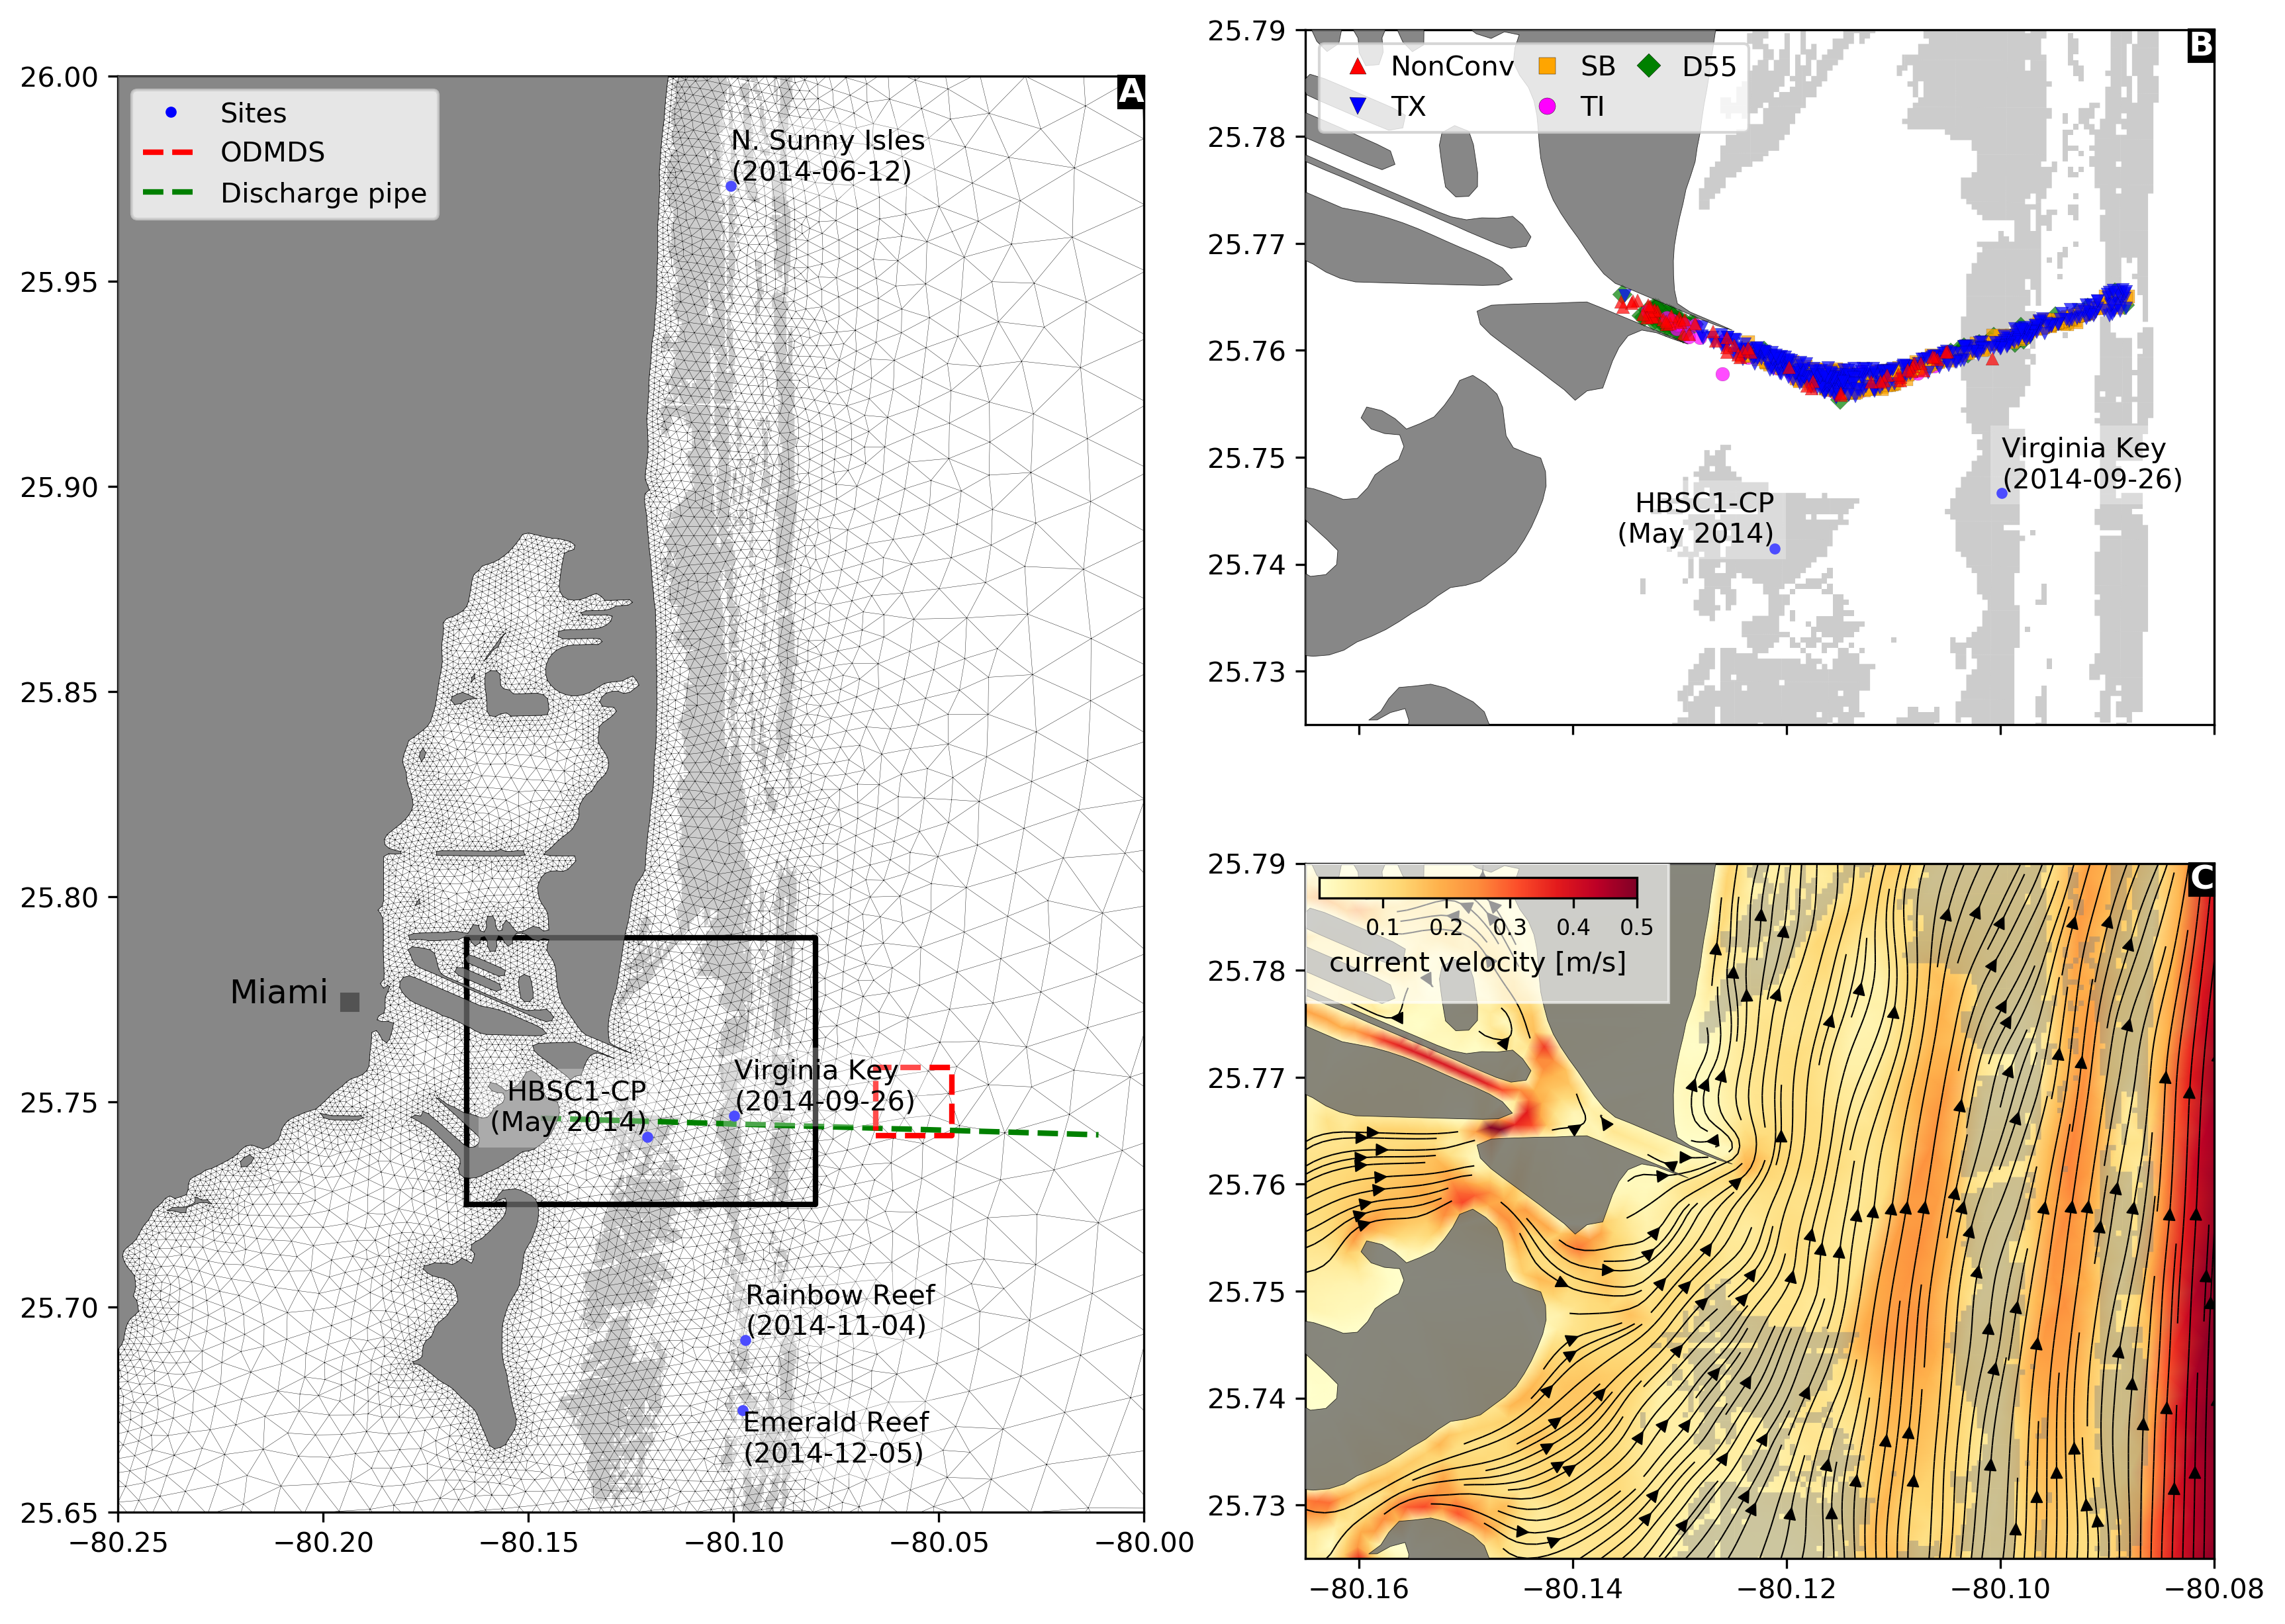
\includegraphics[width=\textwidth]{figures/fig_mesh_onset.png}
    \caption{\textbf{A}: Model mesh near the dredged channel. Elements have a characteristic length of 100 m over reefs (in light grey) and along the coasts (in dark gray). The monitoring sites considered in the present study are shown by blue dots. The date where SCTLD was first observed at these sites is given between brackets. The Ocean Dredge Material Disposal Site (ODMDS) is shown in red. \textbf{B}: Close up view of the dredged channel. The locations of the different types of dredging that took place during the expansion of PoM are shown by colored markers. \textbf{C:} Snapshot of the modeled currents in the vicinity of the dredged channel. Small-scale flow features such as the acceleration of currents between reefs and between islands are well captured by the model.}
    \label{fig:onset_mesh}
\end{figure}

The hydrodynamics of the entirety of FCR was modeled using the high resolution unstructured-mesh model SLIM\footnote{\url{ https://www.slim-ocean.be}}, which has already been extensively validated in the area \citep{frys20,dobbelaere2020coupled,dobbelaere2022}. SLIM uses an unstructured mesh whose resolution can be locally increased in order to accurately represent fine-scale flow features. The mesh used in this study was built following the same methodology as \cite{dobbelaere2022}, with a local refinement near PoM and in the Bay of Biscayne to achieve a resolution of 100 m in the vicinity of the dredged channel (Fig. \ref{fig:onset_mesh}A). It was made up of approximately $3.5\times 10^5$ triangles and was generated with the seamsh\footnote{\url{https://pypi.org/project/seamsh/}} Python library, which is based on the the open-source mesh generator GMSH \citep{geuzaine2009gmsh}. The model was run between October 15, 2013 and September 26, 2014 to cover the whole dredging period prior to the first observation of SCTLD by \cite{precht2016unprecedented}. Figure \ref{fig:onset_mesh}C depicts how a 100-m spatial resolution mesh simulated fine-scale details of the ocean currents, such as the accelerations between reefs and between islands.

The transport of sediments released from the channel was then modeled using a Lagrangian particle tracking model, forced by SLIM velocity field. The sediment model is inspired by the Particle Transport Model (PTM), developed by the US Army Corps of Engineers \citep{macdonald2006ptm}. In this model, particles undergo a combination of horizontal and vertical motions. The vertical is mostly driven by gravity, with heavier particles sinking faster. Once they have settled, particles can be resuspended when shear stress exceed the critical Schields parameter, as parameterized by \cite{soulsby1997threshold}. The horizontal motion of the suspended particles is derived from the 2D model velocity by assuming a vertical log profile, following a quasi-3D approach. When sediment particles enter the near-bed zone, their horizontal velocity is greatly reduced and sediments are transported with the bedload.

As sediment dispersion is dependent on the grain size, we modeled the dispersal of five classes of sediments to represent to impact of fine- to coarse-grained particles: ($i$) 5-50 $\mu$m, ($ii$) 50-100 $\mu$m, ($iii$) 100-200 $\mu$m, ($iv$) 200-300 $\mu$m, and ($v$) 300-400 $\mu$m. We performed a  different simulation for each class, with the grain size randomly drawn from a uniform distribution over the corresponding size range. The density of each sediment particle was derived from their size using the formula of \cite{hamilton1982sound}. Furthermore, all particles were differentiated based on the type of dredge that produced them. Five types of dredge were considered in our modeling study (Fig. \ref{fig:onset_mesh}B): ($a$) Texas cutterhead (TX), ($b$) non-conventional dredging, \ie TX with suction mechanism turned off (NonConv), ($c$) Spider Barge (SB), ($d$) Terrapin Island hopper (TI), and ($e$) Dredge 55 clamshell (D55).

Dredging operations performed during the expansion of PoM were characterized in our dataset by a date, a location and  a type of dredging operation (Fig. \ref{fig:onset_mesh}B). In the absence of information about the exact time of the dredging, sediment particles were released from the dredging location during a whole day at a rate of 80 particles/hour in the model. To account for the motion of spider barges between the dredging site and disposal site, particles were released every 500 m along a straight line joining the dredging location to the ODMDS (see Fig. \ref{fig:onset_mesh}A) for every dredging operation labelled as SB.

To assess the occurrence of high turbidity over reefs, we compared the sediment model outputs against daily data of plume detection. This data set was derived from satellite imagery by \cite{cunning2019extensive} following the methods of \cite{barnes2015sediment} at sites located within 15 km of the dredged channel. As low sediment concentrations might not induce high turbidity levels, we had to define a minimal sediment concentration for the occurrence of plumes in the model. First, the mean daily concentration of modeled sediment particles (particles/m$^2$) was computed by counting the number of sediment particles inside a regular 200 m $\times$ 200 m grid over our computational domain. The daily presence or absence of sediment plumes in a given grid cell was then modeled by evaluating whether the mean daily sediment particle was above (presence) or below (absence) a given threshold. The value of this threshold was obtained by computing the threshold value that best reproduced the plume detection of \cite{cunning2019extensive}. 

We evaluated the impact of dredging at five different sites. Four sites were reefs where disease was reported in 2014 by \cite{precht2016unprecedented}. The fifth site was monitoring station HBSC1-CP of the monitoring of the expansion of PoM, where signs of disease were reported in May 2014 (Fig. \ref{fig:onset_mesh}A) \comment{[Photos in appendix ? ]}. The impact of dredging was assessed by counting the number of sediment particles originating from each dredging that were transported within 500 m of all five site. This number was then divided by the total number of sediment particles released by each type of dredge. Larger values of this indicator would suggest a greater impact of a given type of dredging at a given monitoring sites.

Finally, as previous studies showed evidence of waterborne transmission of SCTLD \citep{aeby2019pathogenesis, dobbelaere2020coupled,eaton2021measuring, meiling2021variable}, there is a possibility that the disease propagated to Virginia Key from other diseased reefs affected prior to September 2014. To evaluate this possibility, we computed monthly disease connectivity matrices following the methodology of \cite{dobbelaere2020coupled} during our simulated period. These connectivity matrices can be interpreted as large graphs whose vertices are sub-areas of reefs and whose edges represent disease connectivity pathways. Evaluating the possibility of disease propagation from any reef $A$ to any reef $B$ is therefore equivalent to evaluating the existence of paths, \ie sequences of connected vertices in the network starting from $A$ and reaching $B$. As computing all possible paths is not computationally tractable, we limited ourselves to the computation of shortest paths from any given reefs to the Virginia Key monitoring site. This was performed using the function \texttt{get\_all\_shortest\_paths} of the Python \texttt{python-igraph} package \citep{csardi2006igraph}. Such function requires the definition of a weight $w_{ij}$ for the edge connecting reef $i$ to reef $j$. We chose $w_{ij} = 1-\tilde{C}_{ij}$, where $\tilde{C}_{ij}$ is the probability of disease propagation from reef $i$ to reef $j$, so that "shorter" edges of the networks (\ie connectivity pathways with smaller weights) correspond to connections with larger disease propagation probability. The probability of a given path was then defined as the mean connection probability of the edges composing this path.

%%%%%%%%%%%%%%%%%%%
% --- RESULTS --- %
%%%%%%%%%%%%%%%%%%%
\section{Results}

The modeled daily presence/absence of sediment plumes agreed well with plume detection from satellite within 15 km of the dredged channel. The model prediction matched plume detection by satellites in about 85\% of the cases for all simulated grain size. As in \cite{cunning2019extensive}, the sediment models predicted plumes 20\% of the simulated days at a distance of 5 km from the dredged channel. However, unlike \cite{cunning2019extensive}, the modeled spatial distribution of plumes was not symmetrically centered around the channel. In our case, plumes occurred more often on the northern side of the channel, as sediments particles tend to drift northward under the influence of the Florida Current (Fig. \ref{fig:onset_depo}). No modeled plumed occurred near Rainbow Reef and Emerald Reef during our simulation. However, the spatial distribution areas of plume occurrence tended to shift southward when the modeled grain size increased. For larger grains, the frequency of modeled plumes increased near Virginia Key and HBSC1-CP and decreased in the vicinity of N. Sunny Isles. The total area of grid cells where plumes were detected during the simulation ranged from 35 to 55 km$^2$, depending in the grain size of the sediments particles.

% \begin{table}
%     \centering
%     \begin{tabular}{|l|cccc|}
%         \hline
%          & Threshold         & Accuracy & False positive  & False negative \\
%          & [particles/m$^2$] & [\%]     & [\%]            & [\%]  \\
%         \hline
%         5-50 $\mu$m    & 21 & 86.678 & 2.912 & 10.410 \\
%         50-100 $\mu$m  & 20 & 83.058 & 8.525 & 8.417 \\
%         100-200 $\mu$m & 30 & 84.814 & 7.133 & 8.053 \\
%         200-300 $\mu$m & 18 & 84.459 & 7.988 & 7.553 \\
%         300-400 $\mu$m & 13 & 84.615 & 8.140 & 7.244 \\
%         \hline
%     \end{tabular}
%     \caption{Validation of the modeled presence of plumes against plume observations from satellite imagery. Overall, the model agrees well with observations}
%     \label{tab:onset_val} 
% \end{table}

\begin{figure}
    \centering
    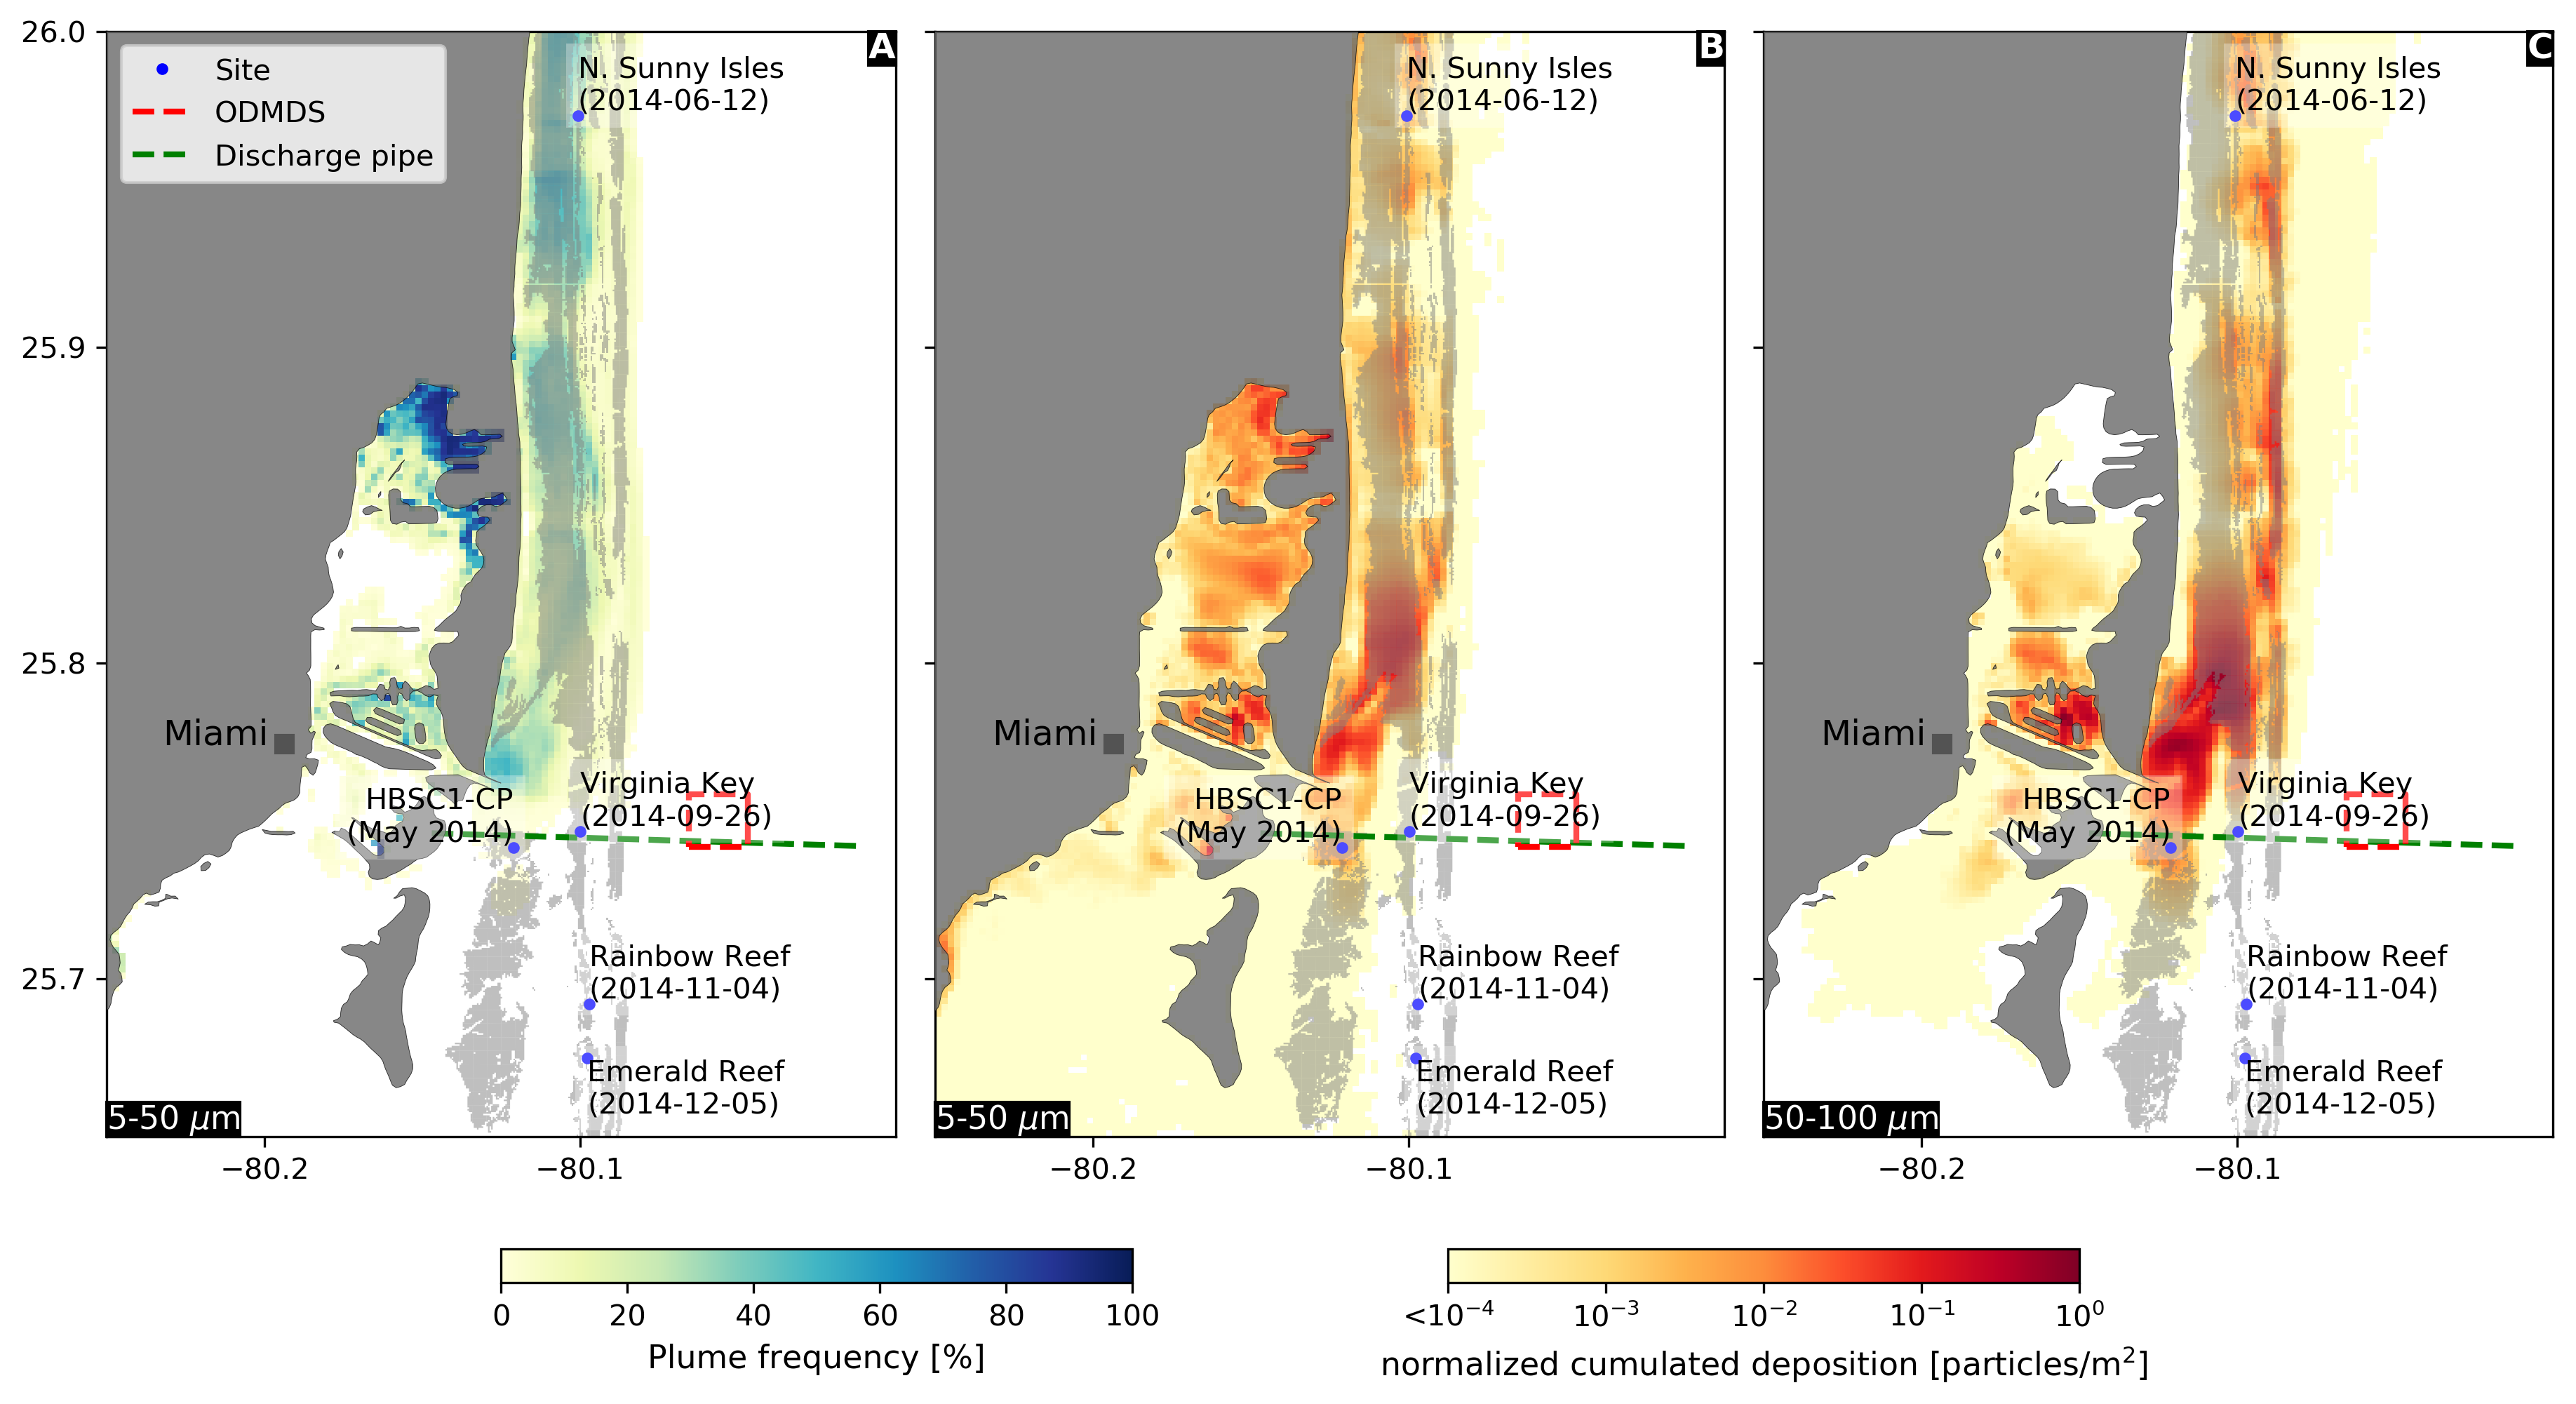
\includegraphics[width=\textwidth]{figures/deposition_plumes.png}
    \caption{Averaged deposited sediment concentration for modeled grain sizes with the highest disease potential: 5-50 $\mu$m (left) and 50-100 $\mu$m (right). Regions where the concentration of suspended sediments exceeded the computed plume threshold are shown by hashed gray areas. Most modeled sedimentation and plumes occurred north of the dredged channel.}
    \label{fig:onset_depo}    
\end{figure}

The impact of sediment deposition on coral reefs was evaluated by dividing the cumulated concentration of deposited particles by the total number of simulation time steps (Fig. \ref{fig:onset_depo}). This produced an estimate of the averaged concentration of settled particles during the simulation. the Deposition results are shown for grain sizes corresponding to silts, which are more likely to carry organic matter and therefore more likely to carry SCTLD agents. Sedimentation mostly occurred on reefs located north of the dredge channel, especially on offshore reefs, while no sedimentation occurred  near Rainbow Reef and Emerald Reef. However, simulated silt particles  deposited at similar latitudes in the Bay of Biscayne. As with plumes, the areas of high modeled sedimentation tended to shift southward for larger grain sizes. Significant sedimentation occurred at site HBSC1-CP for all grain sizes. Sedimentation increased near Virginia Key with larger grain sizes but the site itself remained in an area with limited sediment deposition. Areas of stronger deposition coincided with zones where plumes were detecting, which is consistent with the correlation highlighted by \cite{cunning2019extensive}.

The analysis of the particle trajectories confirmed previous results and indicated that dredging did not significantly impact the reefs located south to the dredge channel, except at site HBSC1-CP (Fig. \ref{fig:onset_bar}). In contrast, up to 40\% of the released sediment particles reached the northern site of N. Sunny Isles. The impact of dredging at this site decreased with sediment size and the fraction of sediment particles reaching the N. Sunny Isles dropped below 2\% for grain sizes larger than 200 $\mu$m. For grain sizes below however, 50 $\mu$m, N. Sunny Isles was heavily impact by TX dredging, with 188,485 particles reaching the site. This is 50\% larger than the cumulated number of particles produced by other dredging operations reaching N. Sunny Isles for the same grain size. Such large impact can be explained by the fact that TX was one of the most frequent type of dredging during the simulations, with 268 simulated operations (Fig. \ref{fig:onset_bar}E). However, SB events occurred at an equivalent frequency but caused 4 times fewer sediment particles to reach N. Sunny Isles. For grain sizes below 100 $\mu$m, between 10\% and 30\% of the sediments released by non conventional dredging reached N. Sunny Isles. This fraction dropped below  1\% for grain sizes larger than 200$\mu$m. The fraction of sediments produced by non conventional dredging reaching site HBSC1-CP remained between 1\% and 5\% for all grain sizes. For grain sizes below 100 $\mu$m, D55 and NonConv were the strongest sources of sediments reaching HBSC1-CP. Above 100 $\mu$m, the strongest source of sediments to the site became TI. The fraction of sediments produced by Spider Barges (SB) reaching HBSC1-CP remained negligible for all grain sizes. No simulated sediment particles reached the sites of Rainbow Reef and Emerald Reef in all simulations. However, some particles reached Virginia Key for grain sizes larger than 100 $\mu$m. These sediments particles almost solely originated from Spider Barges. Nonetheless, the impact of the dredging on Virginia Key remained limited with less than 1$\%$ of the released particles reaching the site.

\begin{figure}
    \centering
    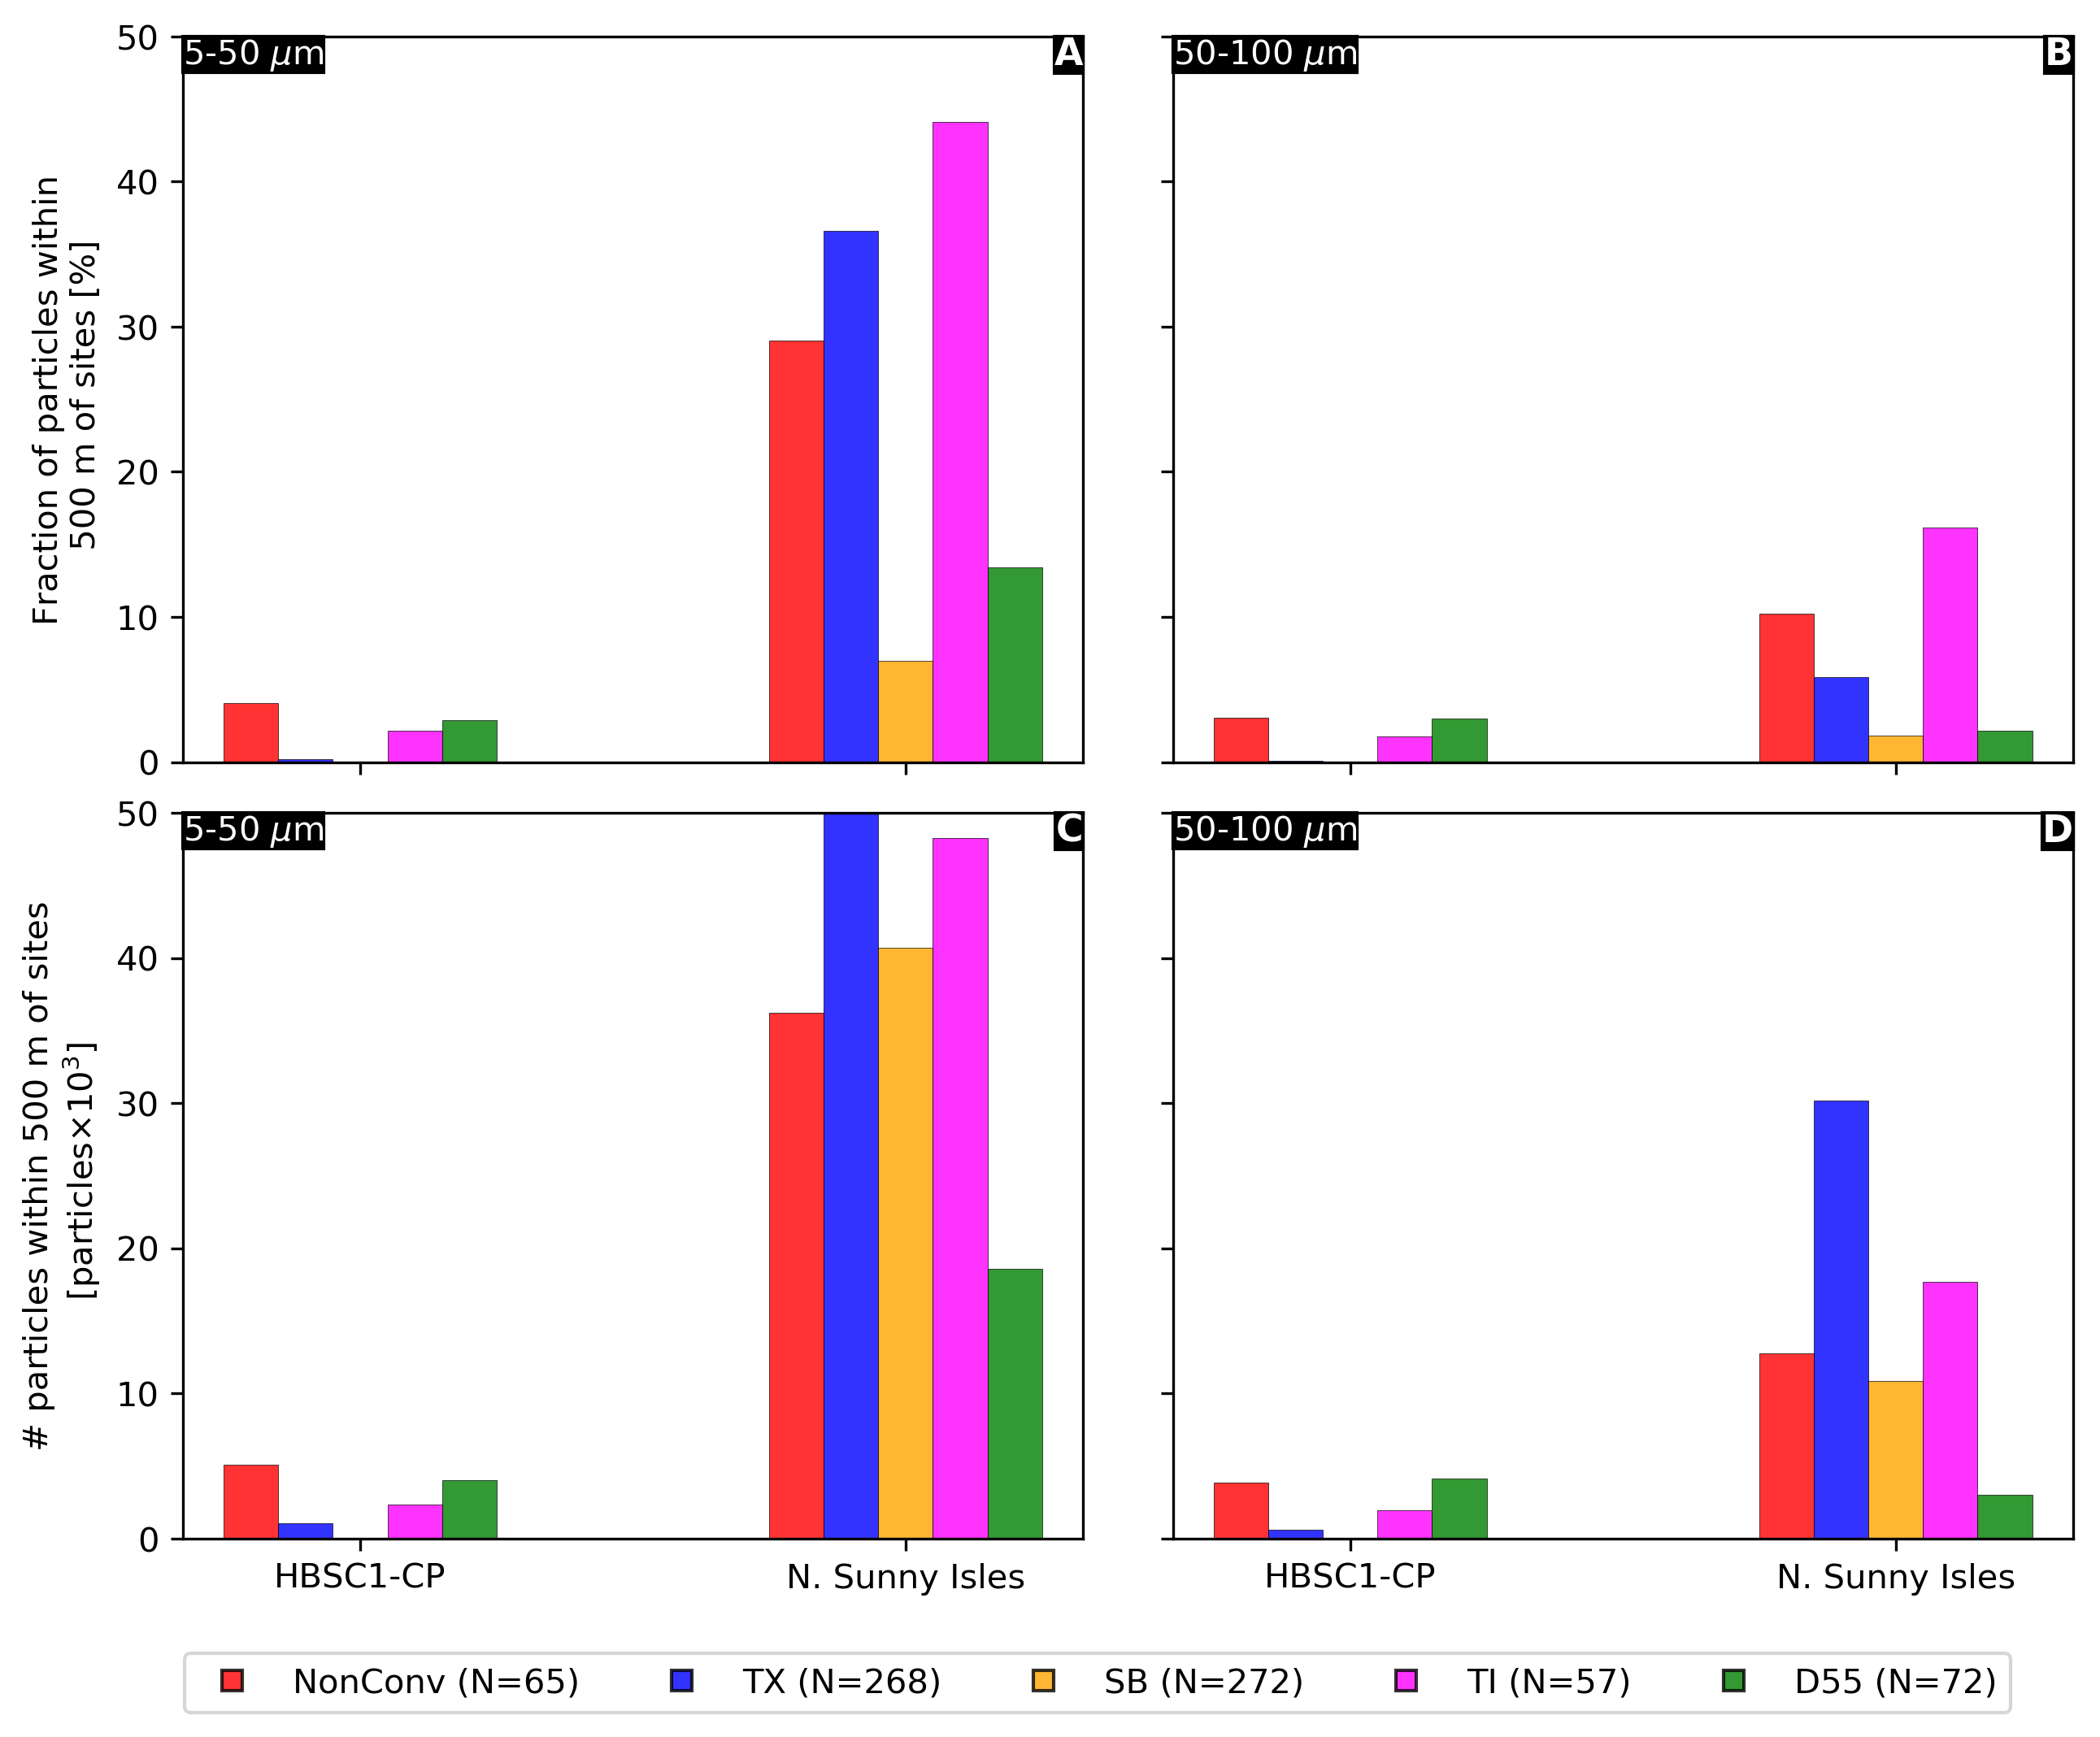
\includegraphics[width=.85\textwidth]{figures/aggregated_with_absolute.png}
    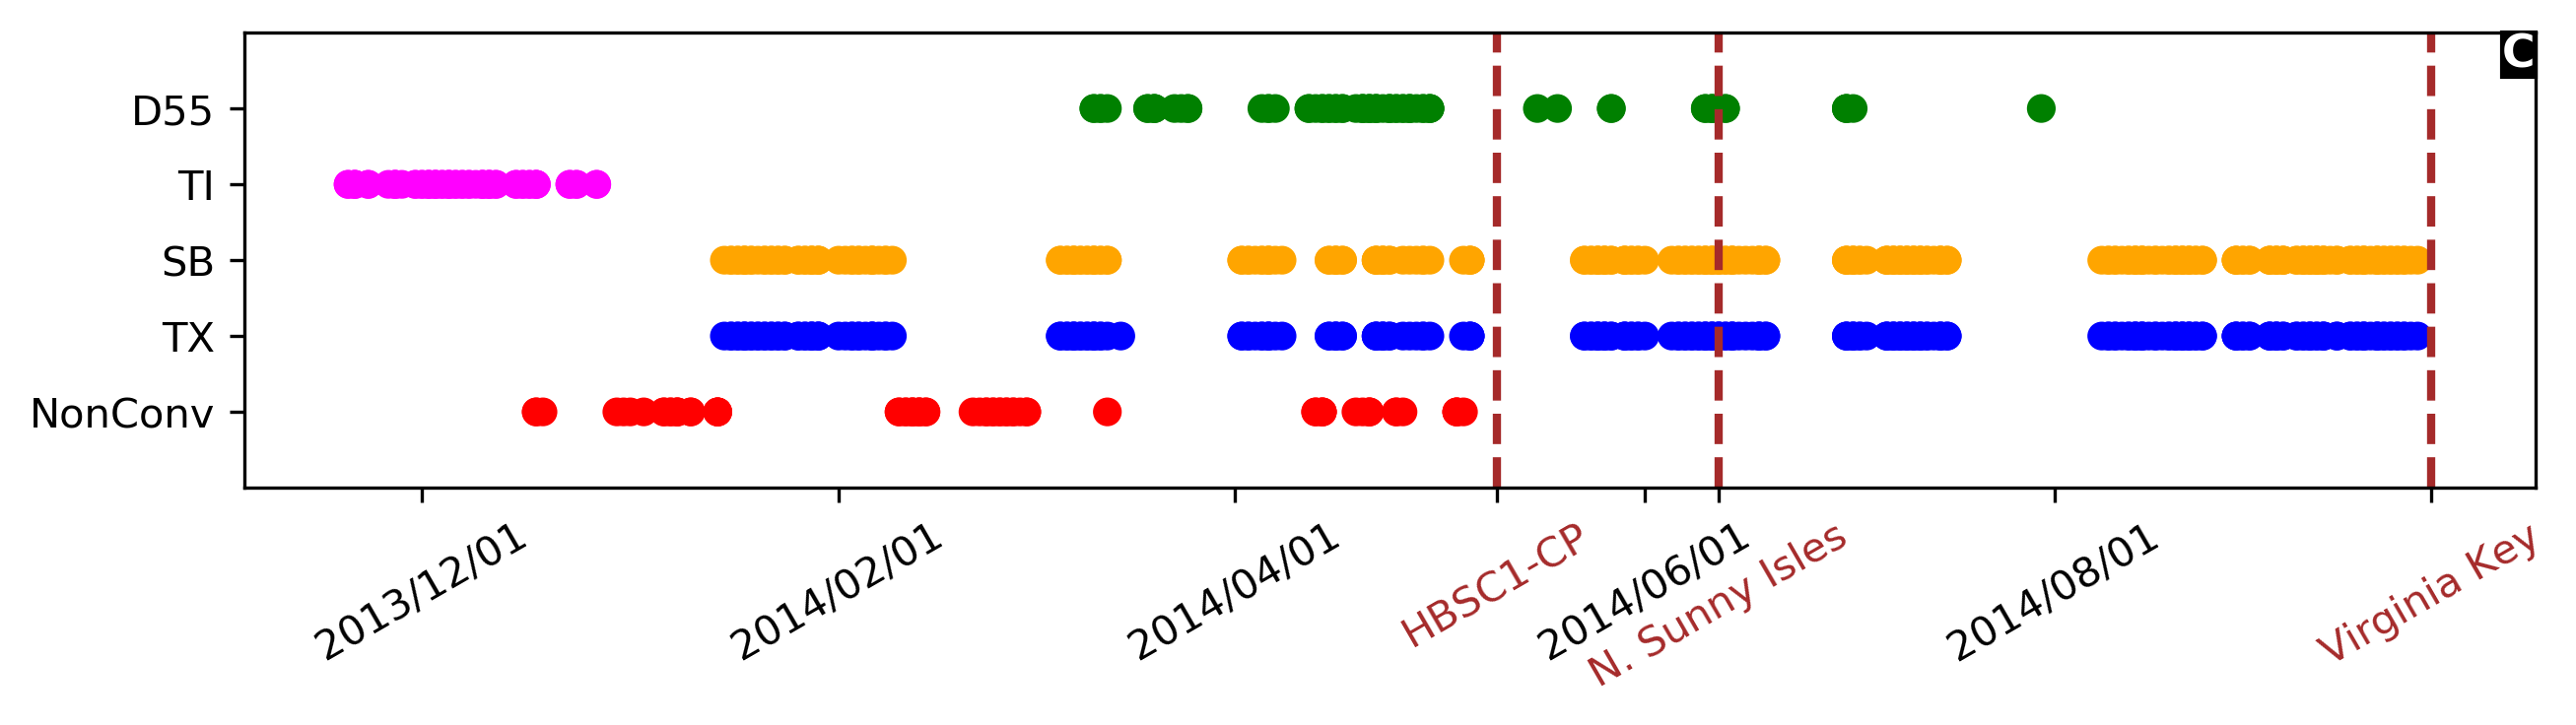
\includegraphics[width=.85\textwidth]{figures/timeline.png}
    \caption{Fraction and absolute number of sediment particles released by each type of dredge that drifted within 500 of HBSC1-CP and N. Sunnny Isles grain sized of 5-50 $\mu$m (\textbf{A},\textbf{C}) and 50-100 $\mu$m (\textbf{B},\textbf{D}). \textbf{E}: Temporal distribution of the simulated dredging operations. With the exception of HBSC1-CP, sites located south to the dredged channel were barely impacted by the dredging. However, a significant fraction of the released sediment particles reached the northern site of N. Sunny Isles, with 188,485 sediment particles produced by TX for grain sizes in the range 5-50 $\mu$m. The number of simulated dredging operations is given between brackets for each dredging type}
    \label{fig:onset_bar}
\end{figure}

As signs of disease were observed at site HBSC1-CP in May 2014, before the first observations of SCTLD in Virginia Key in September 2014, we assessed the presence of shortest paths from HSC1-CP to Virginia Key in the modeled monthly disease connectivity networks between May and September 2014 (Fig. \ref{fig:onset_path}). We found connectivity pathways connecting the two sites during all months of May-September 2014, except July 2014. This suggests that there was a possibility of disease propagation from HBSC1-CP to Virginia Key during most of these 5 months. However, we found no direct pathway connecting the two sites. Southern intermediary reefs were systematically needed as stepping stones for the propagation of the disease. This suggests that several months might have been required for disease agents to reach Virginia Key from HBSC1-CP. Moreover, shortest paths in June, August and September 2014 had many sub-reef stepping stones in common. These similar connectivity patterns indicate favorable conditions for disease propagation over several months from HBSC1-CP to Virginia Key during this period.  

\begin{figure}
    \centering
    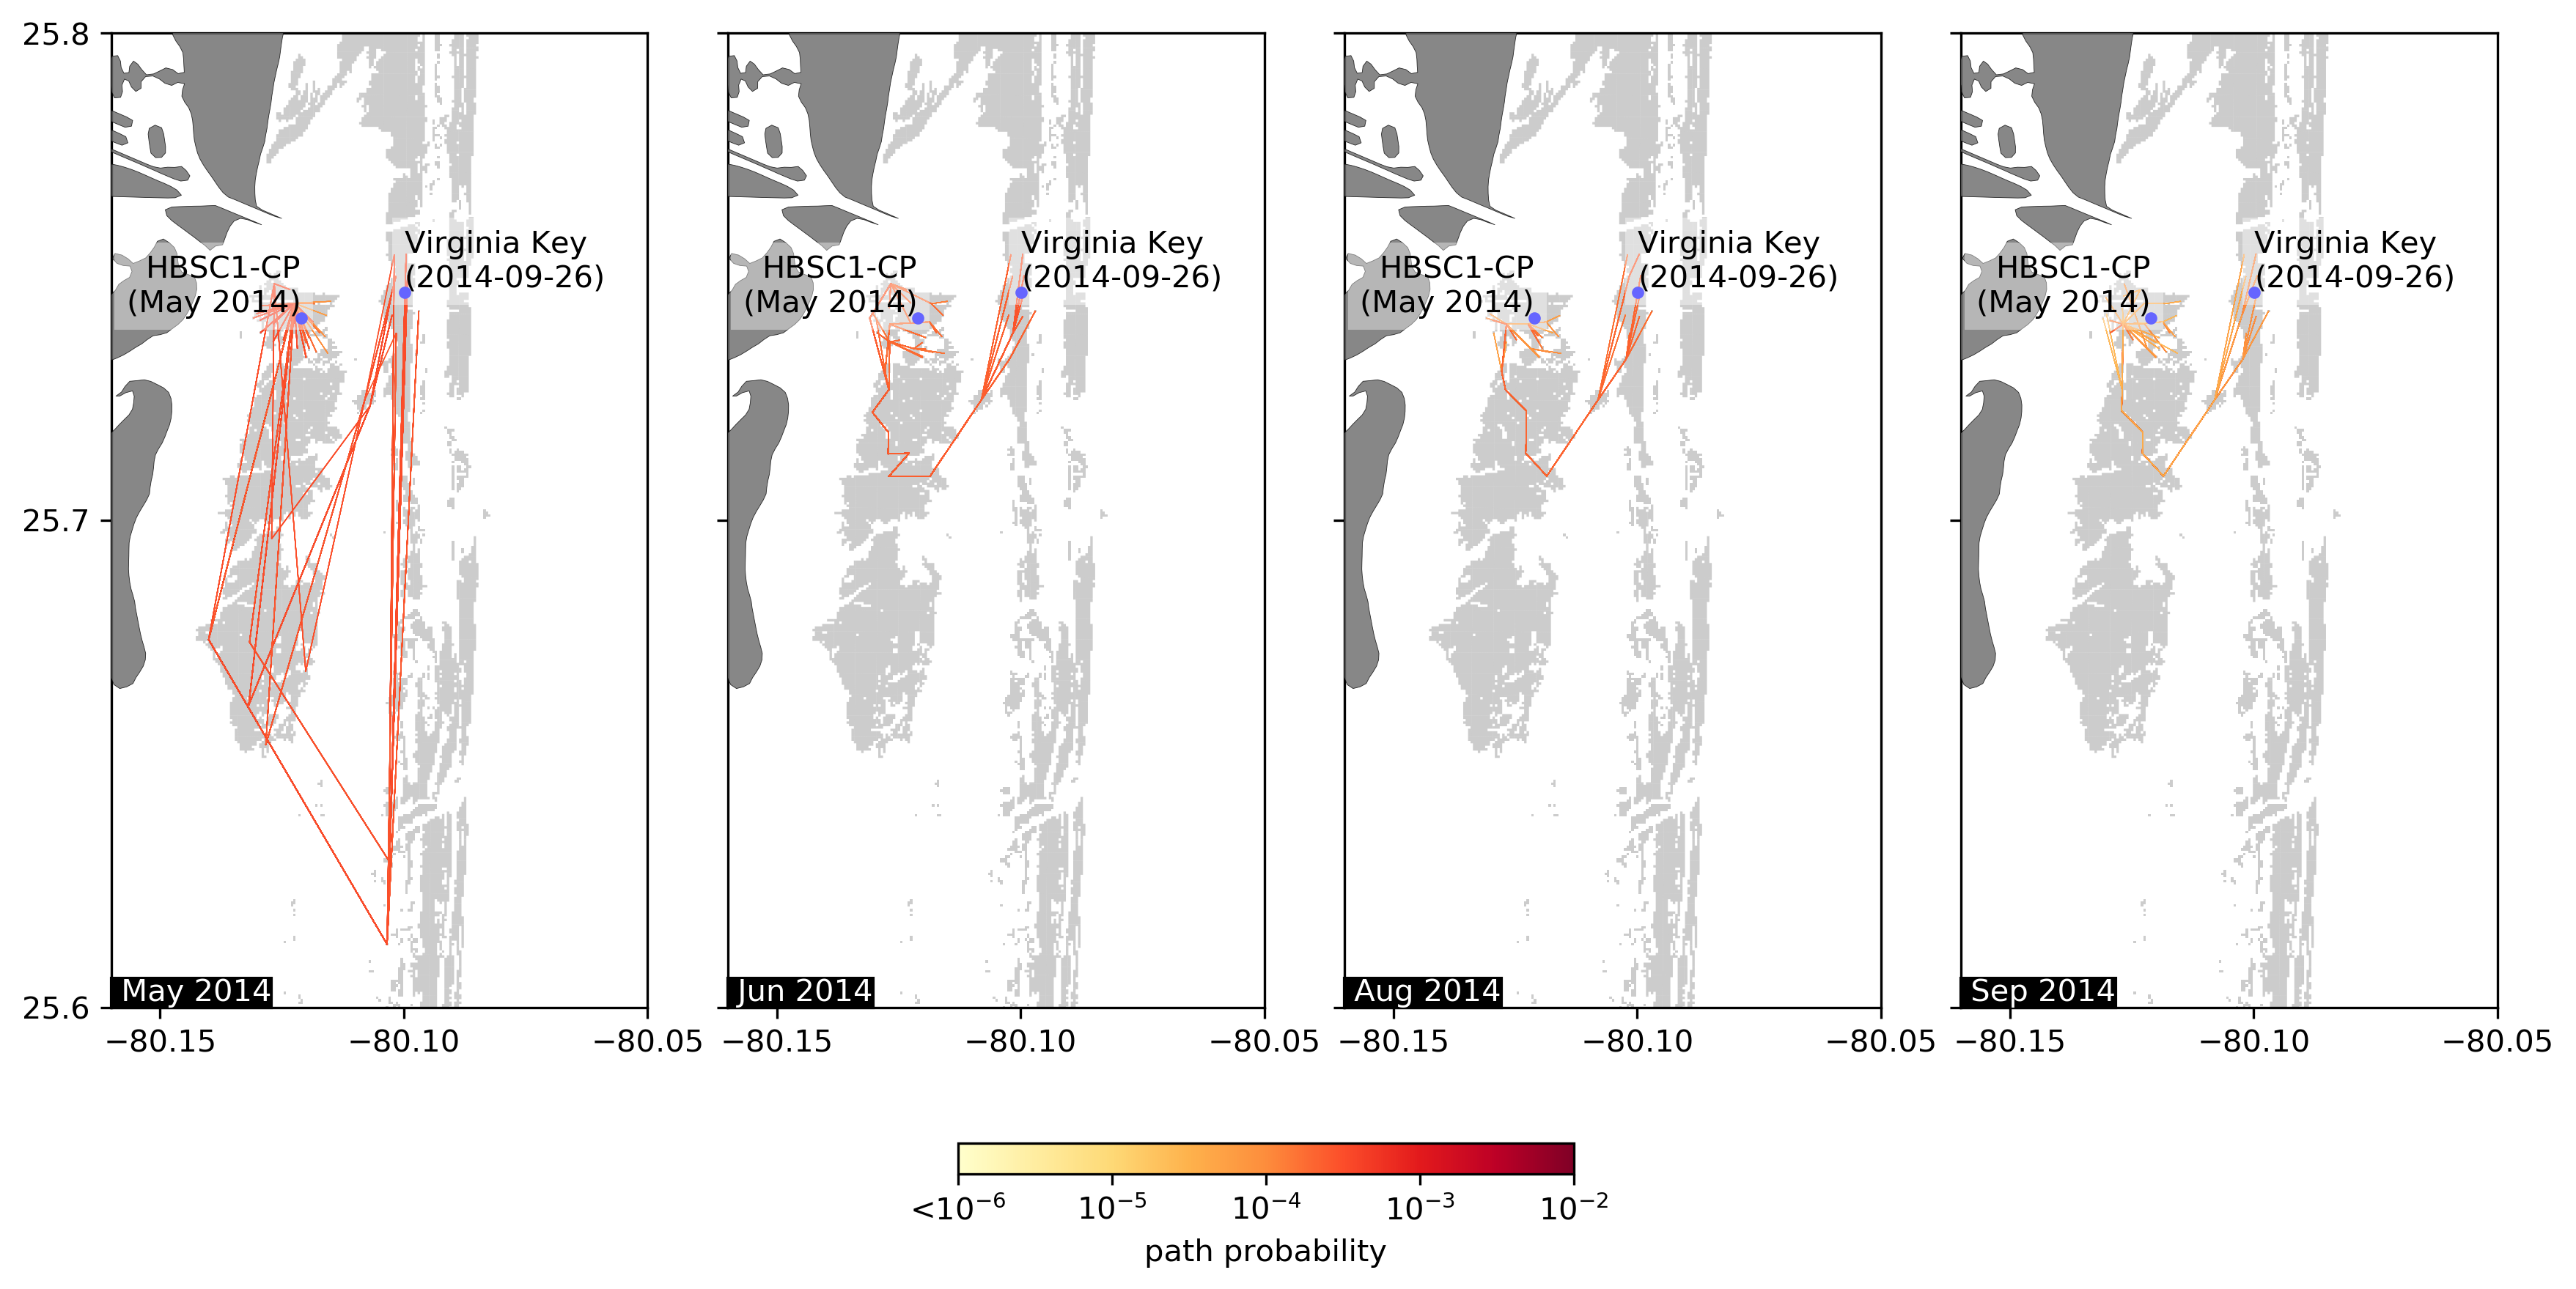
\includegraphics[width=\textwidth]{figures/fig_paths.png}
    \caption{Shortest path from HBSC1-CP to Virginia Key in the monthly disease connectivity networks between May and September 2014. July 2014 was the only month without modeled connectivity between the two sites between May and September 2014. Southern intermediary reefs were needed as stepping stones for the propagation of the disease from HBSC1-CP to Virginia Key.}
    \label{fig:onset_path}
\end{figure}

\todo{Section about discharge pipeline}

\begin{figure}
    \centering
    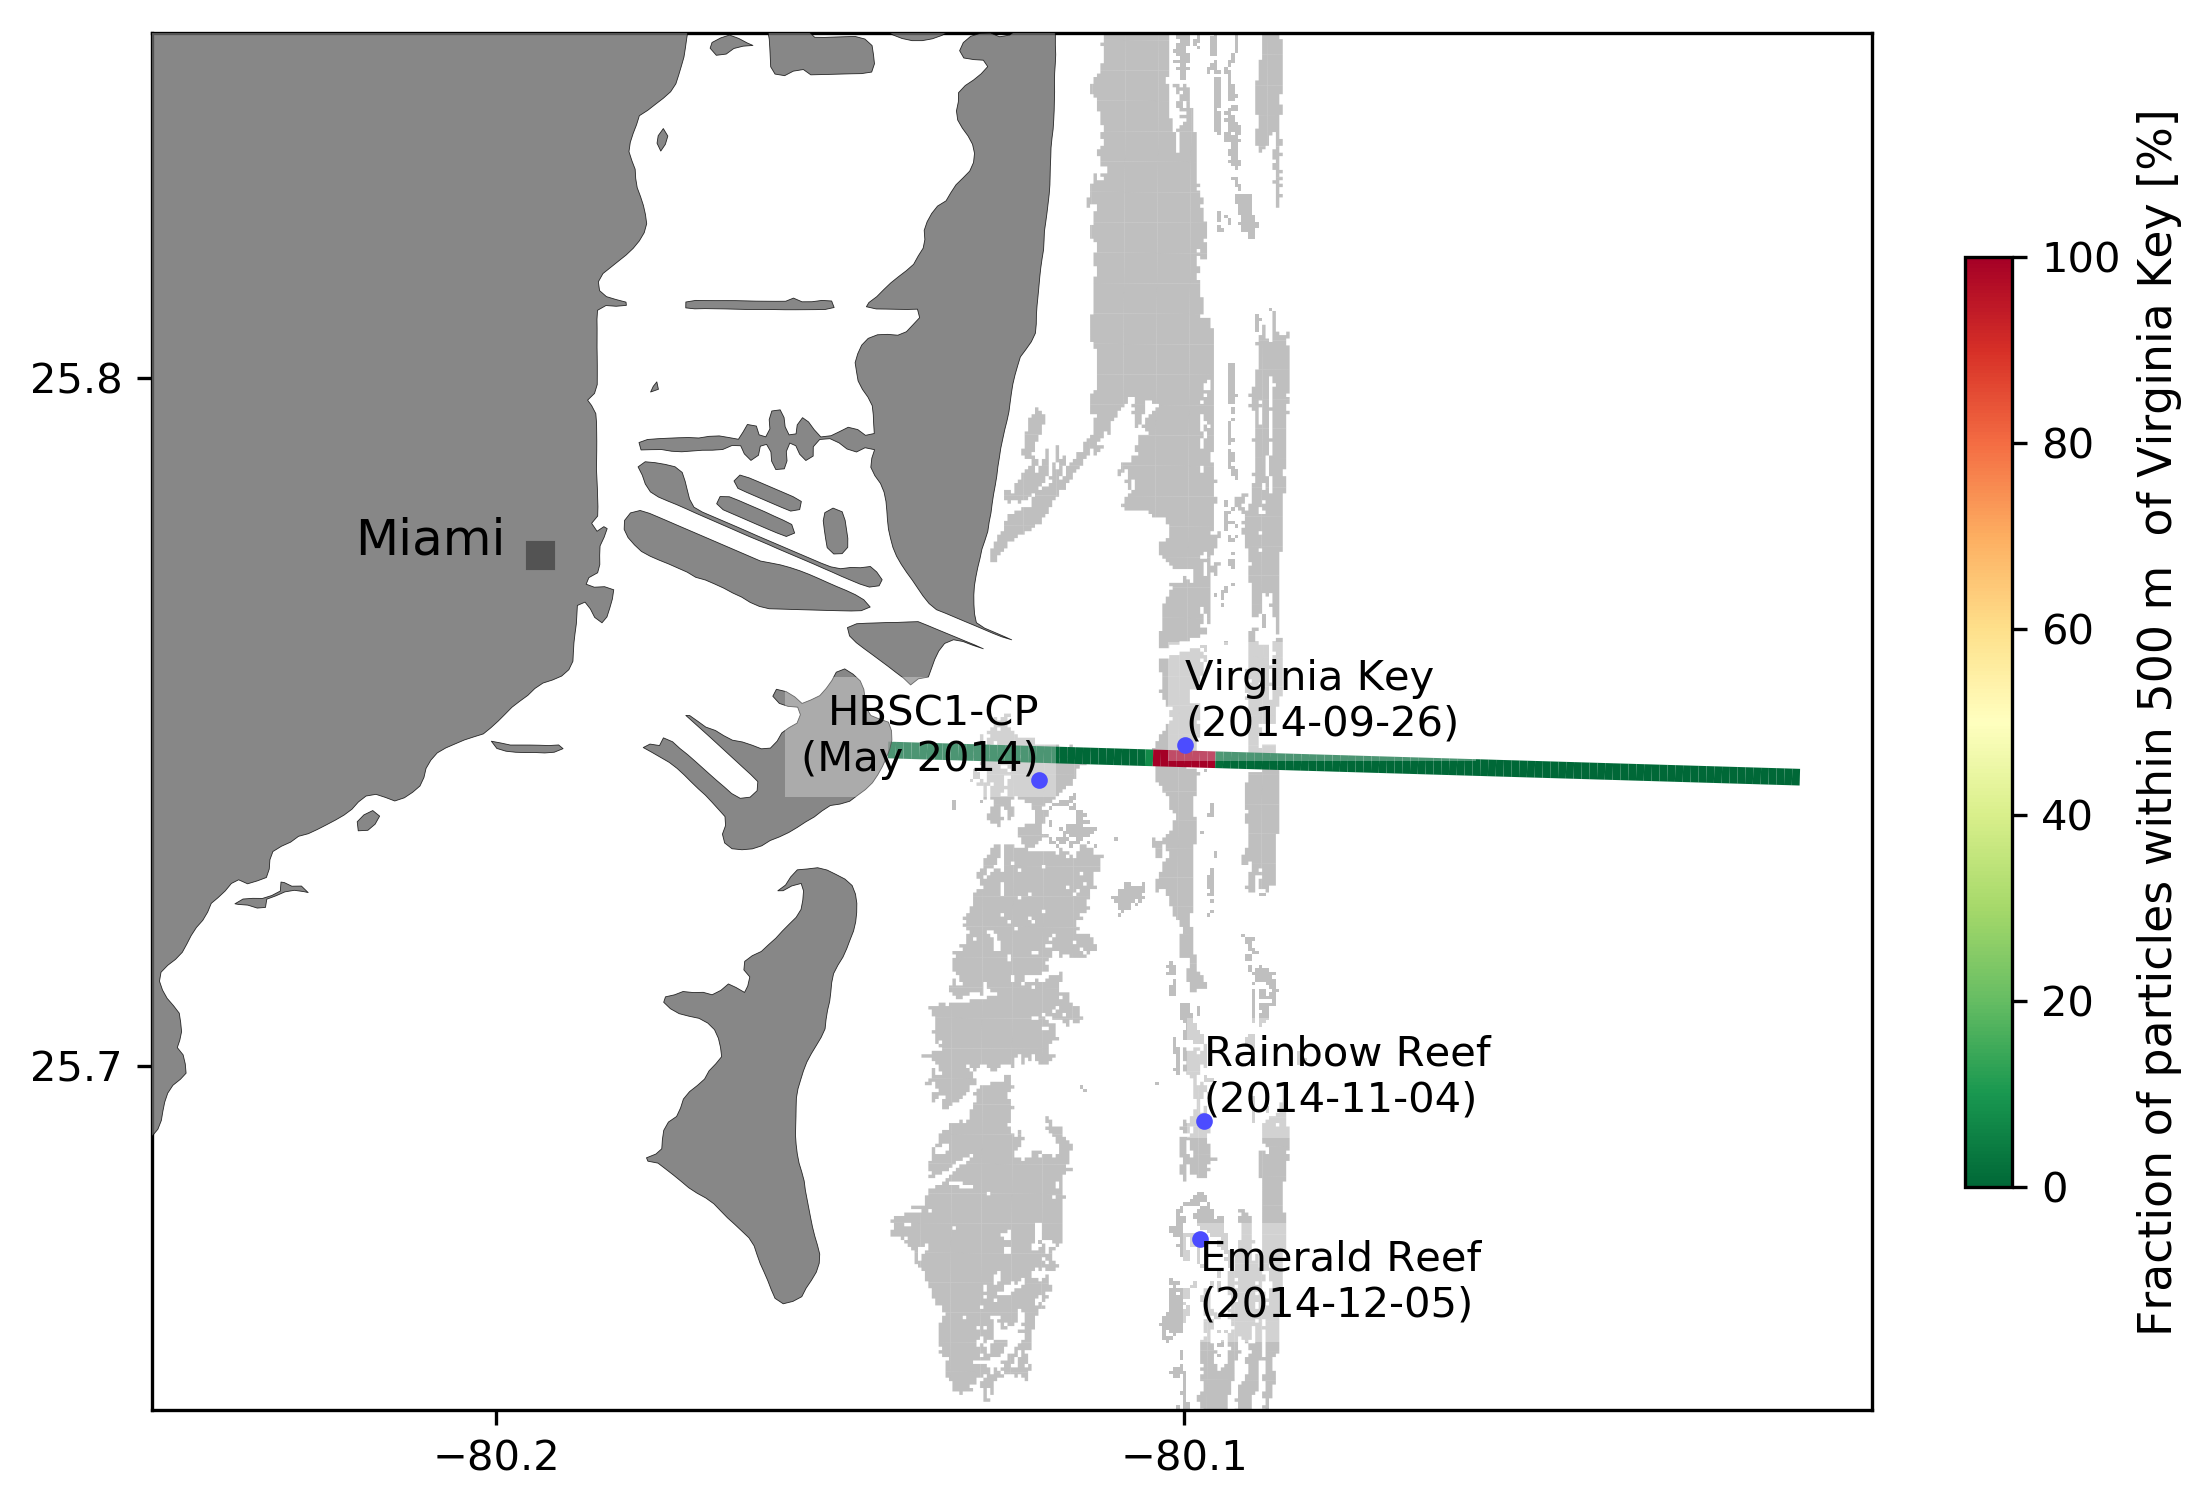
\includegraphics[width=.7\textwidth]{figures/pipeline.png}
    \caption{\todo{description}}
    \label{fig:onset_pipe}
\end{figure}


% === DISCUSSION === %
\section{Discussion}
\todo{Insist more of non conv dredging}

The quasi-3D sediment model forced by currents from the high-resolution coastal ocean model SLIM reproduced sediment dynamics consistent with plume observations derived from satellite imagery. It suggests that sediment particles produced by dredging were mostly transported northward under the influence of the Florida Current. Between 10\% and 40\% of silts produced by non-conventional dredging could have reached coral reefs of N. Sunny Isles. No sediment particles reached the sites of Rainbow Reef and Emerald Reef. For all simulated grain sizes, the fraction of sediments reaching HBSC1-CP remained between 2\% and 5\%. In all simulation, dredging had close to no direct impact of Virginia Key, with less than 1\% of the coarser ($> 100$ $\mu$m) sediment particles reaching the site. Nonetheless, analysis of the monthly disease connectivity matrices show that disease propagation from HBSC1-CP to Virginia Key in May, June, August and September 2014.

This study confirms previous reports about the widespread impact of the expansion of PoM \citep{barnes2015sediment,miller2016detecting,cunning2019extensive}, with sediment particles depositing more than xx km away from the dredged channel. However, the extent of sediment plumes was at most 55 km$^2$, which is way below the $\sim228$ km$^2$ estimated by \cite{barnes2015sediment}. These discrepancies might be explained by the fact that our approaches is solely based on sediment concentration. However, turbidity depends on many local factors such as the water content phytoplankton organic matters \citep{gray2000comparability,thackston2000improved}. Plume areas might therefore be underestimated in our model. Nonetheless, plume detection based on sediment particle was grain-size specific in our model and gave results consistent with \cite{cunning2019extensive} within 15 km of the dredged channel.

A limitation of our study is that the amount released sediments might be overestimated, as conventional and non-conventional dredging are treated in the same way in the model. For all dredging types, sediment particles were released at the same rate in the model. Although conventional dredging was reported to release fine-grained sediments in the water column through dewatering and overflow from barges \citep{jones2016assessing}, the quantity of dredged material lost in the water was limited by the use of pumping mechanisms. By contrast, for non-conventional dredging, the suction mechanism was turned off, causing all chopped rocks to be released in the water column. The numbers of particles reaching the monitoring sites shown in Fig. \ref{fig:onset_bar}C,D were therefore likely overestimated for all sources but non conventional dredging. However, the fractions given in Fig. \ref{fig:onset_bar}A,B remain valid as they are relative to the total number of sediments released in the water columns. Despite these overestimations, the coral reefs of N. Sunny Isles appeared to be highly sensitive to fine-grained sediments produced by the dredging (Fig. \ref{fig:onset_bar}). Furthermore, the non-conventional rock-chopping that took place between December 2013 and May 2014, was a non-negligible source of sediments to N. Sunny Isles, as up to 30\% of the released particles reached the site. As sediments have the potential to act as a SCTLD vector \citep{rosales2020rhodobacterales, studivan2022reef}, the dredging might therefore have contributed to the observed onset of the disease on the reefs of Sunny Isles in June 2014. Moreover, up to 5\% of the fined-grained sediments produced by non-conventional dredging reached the site HBSC1-CP. Although this represents a more limited quantity of sediments, HBSC1 was located about 2 km away from the sites where non-conventional dredging took place, in a region where the model predicted an important sedimentation. Therefore, although fewer sediments reached HBSC1-CP, they had a higher probability to settle and to be in direct contact with corals. In addition to smothering corals and diverting their energy through sediment removal \citep{erftemeijer2012environmental}, these settled sediments are more likely to transmit the disease to the reefs.

In all simulations, the expansion of PoM had no direct impact to Virginia Key, identified as the site where the outbreak initiated in September 2014 \cite{precht2016unprecedented}. For all grain sizes, the fraction of sediment particles reaching Virginia Key remained below 1\%. It is therefore unlikely that sediments produced by the deepening of the channel brought the disease to the site. However, signs of disease were observed prior to September 2014 at the sites of N. Sunny Isles and HBSC1-CP, both of which were impacted by the dredging. Several studies showed evidence of waterborne transmission of SCTLD \citep{aeby2019pathogenesis,dobbelaere2020coupled,eaton2021measuring,meiling2021variable}. Disease agents might therefore have been transported by currents from one of the diseased sites to Virginia Key. As site HBSC-CP was closest to Virginia Key, we built and analyzed monthly disease connectivity networks and found connectivity pathways from HBSC1 to Virginia Key in May, June, August and September 2014. This implied that the propagation of the disease from HBSC1-CP to Virginia Key through hydrodynamics-driven transport of disease agents was possible during these four months. However, these pathways used reefs located further southward as stepping stones. Therefore, the propagation of outbreak to reach Virginia Key starting from HBSC1-CP required these intermediary reefs to get first infected by disease agents released by disease colonies of HBSC1-CP. Once diseased, these colonies would then send diseased agents to affect the next colonies of the connectivity pathway until the outbreak reached Virginia Key. Assuming an averaged transmission time of the order of 5-10 days \citep{dobbelaere2020coupled}, disease propagation from HBSC1-CP to Virginia Key might have required several months. This is consistent with the 5 month period separating reports of diseased at the two sites. Moreover, the fact that June, August and September exhibited similar connectivity pathways suggests that disease propagation could indeed have occurred over several months without being interrupted by changing hydrodynamic conditions.

\section{Conclusion}


\bibliographystyle{elsarticle-harv} 
\bibliography{./biblio.bib}

\end{document}
\endinput